
\subsection{ESB}
\label{esb:introduccion}

%hablar de IAE

Uno de los 9 principios de diseño de \gls{acro:soa} es el bajo acoplamiento (\eng{loose coupling}) de los servicios.  La forma más común de implementar bajo acoplamiento para los servicios \gls{acro:soa}, es mediante un \gls{acro:esb}.
\todo{ver si se trataron los 9 principios en SOA}
% http://simplicable.com/new/the-9-principles-of-soa-design

Pero que es un \gls{acro:esb}?

Un \gls{acro:esb} no implementa en sí mismo una arquitectura orientada a servicios (\gls{acro:soa}), sino que proporciona las características, mediante las cuales sí puede implementarse.  Proporciona una capa de abstracción para los \eng{endpoints}, de esta manera se consigue flexibilidad y una fácil conexión entre los servicios.

Existen diferentes opiniones acerca del rol exacto y de las responsabilidades de un \gls{acro:esb}.  Parte de esta razón, es que hay diferentes aproximaciones técnicas para realizar un \gls{acro:esb} \cite[p.~47]{josuttis2007}.

En función de los enfoques técnicos y de organización adoptadas para la aplicación del \gls{acro:esb}, puede implicar las siguientes tareas:

\begin{itemize}
  \item Providing connectivity
  \item Data transformation
  \item (Intelligent) routing
  \item Dealing with security
  \item Dealing with reliability
  \item Service management
  \item Monitoring and logging
\end{itemize}

El rol principal de un \gls{acro:esb}, es proveer interoperabilidad.  Debido a que integra diferentes plataformas y lenguajes de programación, una parte fundamental de esta función es la transformación de datos.
Otra tarea fundamental de un \gls{acro:esb}, es el ruteo, debe existir alguna manera de acceder a un servicio desde un consumidor a un proveedor, y luego enviar la respuesta de vuelta desde el proveedor hasta el consumidor.
Dependiendo de la tecnología utilizada, y el nivel de inteligencia proporcionada, esta tarea puede ser trivial, o puede requerir procesamiento muy complicado.

Hay que tener en cuenta que no existe requerimiento alguno para que el \gls{acro:esb} sea homogéneo.  Aunque podría ser mejor usar una sola tecnología para la implementación de los servicios, raramente es el caso. \gls{acro:soa}, por su propia naturaleza, acepta heterogeneidad. Eso incluye la heterogeneidad en middleware y protocolos. Incluso con un estándar como web service, múltiples instancias pueden diferir.  Tarde o temprano, se introducirá un nuevo estándar o una nueva versión del estándar que hace las cosas mejor y más fácil. Tan pronto como empiece a utilizar el nuevo estándar (junto a la antigua tecnología), el \gls{acro:esb} se volverá heterogéneo\cite[p.~49]{josuttis2007}.

Idealmente, el cambio de tecnología en el \gls{acro:esb}, no debe tener ningún impacto en los proveedores y consumidores, deben ser capaces de utilizar la misma \gls{acro:api}, y sólo debe cabmiar el mapeo.
Es decir, desde el punto de vista de los proveedores y consumidores, la \gls{acro:api} de servicios debe ser transparente. Sin embargo, esto por lo general requiere que el \gls{acro:esb} incluya la \gls{acro:api} de servicios para cualquier plataforma específica. Si el \gls{acro:esb} requiere un sólo protocolo específico, los consumidores y proveedores tienen que lidiar con las modificaciones de este protocolo\cite[p.~50]{josuttis2007}.

% hablar de conexiones ponit to point

En la década pasada, nuevos estándar como SOAP aparecieron en escena, estos estándar establecen las bases para aplicaciones interoperables, con el concepto de web services.
Tecnologías como web service, abrieron muchas posibilidades pero tambien trajeron nuevos desafíos.  Uno de estos desafíos es la proliferación de comunicaciones punto a punto entre sistemas.  Esta proliferación a menudo conduce a un modelo de integración llamado ``plato de espaguetis'', con relaciones muchos a muchos entre diferentes aplicaciones.
Aunque el problema de interoperabilidad se resolvió, era complicado su mantenimiento.\cite[p.~4]{dossotandemic2010}.

\begin{figure}[H]
  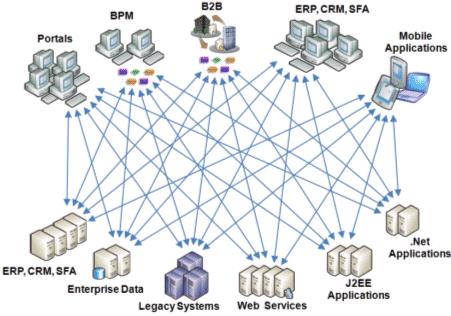
\includegraphics[width=\linewidth]{src/images/03-capitulo-3/tecnologias/esb/point-to-point-integration.png}
  \caption{Integración punto a punto}
  \label{fig:point-to-point-integration}
\end{figure}


% página 50 SOA in Practice - 5.3.1 Point-to-Point Connections Versus Mediation
% agregar figua con topología de interconexión entre aplicaciones, topología en malla

En una arquitectura en la que se implemente un \gls{acro:esb}, las aplicaciones se comunicarán a través del bus, que actúa como \eng{message broker} entre las aplicaciones. De esta manera se reduce el número de conexión punto-a-punto que se necesitan para permitir que se comunique una aplicación con otra.  Al reducir el número de puntos de contacto entre las diferentes aplicaciones, se simplifica el proceso de mantenimiento y actulización de un sistema.

% ver si es necesario desarrollar previamente el tema

Interceptors
La otra forma donde un \gls{acro:esb} basado en un protocolo de punto a punto puede soportar llamadas de servicio indirectas, es proporcionando los llamados ``interceptors'' o ``proxies''. Un enfoque sencillo, es reemplazar el \eng{endpoint} físico que ofrece el servicio, con \eng{hardware} o \eng{software} que sirve como balanceador de carga. Los consumidores siguen utilizando un \eng{endpoint} oficial, donde se delega la verdadera tarea, cuando los mensajes llegan, el balanceador de carga los envía a los diferentes proveedores de servicios que conoce.\cite[p.~52]{josuttis2007}.

\begin{figure}[H]
  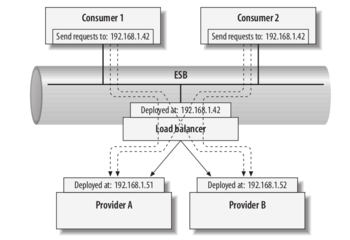
\includegraphics[width=\linewidth]{src/images/03-capitulo-3/tecnologias/esb/esb-interceptors-load-balancer.png}
  \caption{Un ESB con balanceador de carga para los proveedores de servicios}
  \label{fig:esb-interceptors-load-balancer}
\end{figure}
